\chapter{Theory}
\label{chap:theory}

\epigraph{\textit{Dreaming a thought that could ~\\
                  dream about a thought ~\\
                  That could think of the ~\\
                  dreamer that thought ~\\
                  That could think of dreaming and ~\\
                  getting a glimmer of God}
                 }{Frank Ocean}

\section{Introduction}

The standard model (SM) of particle physics is the current best description of nature 
at its most fundamental level.
Developed in the 1970s, the SM incorporates the electromagnetic, weak, 
and strong forces in a single coherent framework, 
unifying the electromagnetic and weak interactions in doing so.
The SM is a type of quantum field theory known as a gauge theory, 
which represents the fundamental constituents of matter and the forces between them
as excitations of relativistic quantum fields.
Many of its predictions have been experimentally verified to unprecedented precision~\cite{EMstuff}.
The spontaneous breaking of gauge symmetry in the unified electroweak (EW) sector of the SM
results in the prediction of the Higgs boson, 
the existence of which is now experimentally confirmed~\cite{HiggsShit}.
In this chapter, the fundamental particles and forces making up the SM are described, 
before its structure as a gauge field theory is explained.
The origin of the Higgs boson and through spontaneous symmetry breaking is elucidated.
The phenomenology of the Higgs boson and the consequences for experimental measurements 
are then detailed. 
Lastly, the simplified template cross section (STXS) framework is introduced 
and the latest precision measurements of the Higgs boson's properties are summarised.

\section{Fundamental particles and forces}

In the SM, particles particles other than the Higgs boson are divided into spin-half fermions
and spin-one bosons.
Fermions are the fundamental constituents of matter, 
and can either interact only via the electroweak force (leptons), 
or via both the electroweak and strong forces (quarks).
Both leptons and quarks exist in three distinct generations;
the three particles comprising each group have identical properties 
except for mass, which increases across generations.
This structure is shown in Table~\ref{tab:theory_fermions}, 
which shows the charge and mass of each type of fermion in the SM.
In addition, each particle has a corresponding antiparticle, 
which have the same mass but whose charge has the opposite sign to the original particle.
%Leptons are exist as free particles but quarks are confined to composite objects 
%such as the proton due to the nature of the strong force.

%TODO insert fermion table here

The interactions between fermions are mediated by a second class of fundamental particles, 
the gauge bosons.
Three forces are represented by the SM gauge bosons: 
the electromagnetic force, the weak nuclear force, and the strong force.
The mediator of the electromagnetic force is the massless photon, 
whilst the weak interaction is occurs via the exchange of three massive particles, 
the $W^+$, $W^-$, and $Z$ bosons.
Due to the unification of these two forces into the electroweak sector of the SM, 
the photon, $W^\pm$, and $Z$ bosons arise from combinations of the fundamental gauge fields.
Gluons, which mediate the strong force, 
are also massless.
%Together these describe all the fundamental forces observed in nature, 
%with the exception of gravity.
The structure of the gauge bosons in the SM is summarised in Table~\ref{tab:theory_bosons}.

%TODO insert boson table here

The final particle in the SM is the Higgs boson, 
which is the only scalar (spin-zero) particle in the theory.
The Higgs boson is a massive particle which arises 
due to spontaneous symmetry breaking in the electroweak sector, 
and whose existence is necessary to explain the masses of both bosons and fermions.

\section{Gauge fields}

The SM is realised as a particular type of quantum field theory (QFT) known as a gauge field theory.
The dynamics and predictions of a given QFT can be derived from the Lagrangian (\Like)
using the Euler-Lagrange equations, 
in the same way as the equations of motion can be derived in classical field theory~\cite{Peskin}.
Typically a Lagrangian is constructed with the aim of respecting symmetries of the physical system
it is attempting to describe.
According to N\"other's theorem~\cite{Nother}, 
each symmetry of a Lagrangian has a corresponding current which is conserved.
Examples include the invariance of a Lagrangian under translations in time 
corresponding to the conservation of energy, 
and invariance under spatial translation to conservation of momentum.
This theorem therefore illustrates that the symmetries of a Lagrangian 
are intimately linked with the conserved quantities and properties of the physical system described.

The defining feature of gauge field theories is that they require the Lagrangian 
to be invariant under a local gauge transformation.
Here a local transformation means one which depends on spacetime co-ordinates, 
in contrast to a global transformation.
Elevating a global symmetry to a local one requires the introduction of additional fields, 
which enable interactions between particles and imply the existence of gauge bosons.
This is illustrated below, starting with the Dirac lagrangian 
which describes a free spin-half fermion~\cite{Dirac,Griffiths}:
\begin{equation}
The Dirac equation
\end{equation}
where... 
The Dirac Lagrangian is invaraint under a global phase transformation 
corresponding to the $U(1)$ group, i.e. 
\begin{equation}
Global transformation
\end{equation}
where...
This invariance is dependent upon the commutation of the transformed field 
with the differential operator. 
Considering instead a local gauge transformation, 
meaning the transformation is a function of the spacetime co-ordinates:
\begin{equation}
Local transformation
\end{equation}
where...,
The Lagrangian is no longer invariant;
instead there is a residual term remaining af
\begin{equation}
Lagrangian transform
\end{equation}
where... 
In order to restore gauge invariance, a new field $A_{\mu}$ can be introduced 
which transforms as
\begin{equation}
Transformation of the photon field
\end{equation}
where... %equiv to a 1x1 matrix / U(1)
This field is incorporated into the definition of the covariant derivative
\begin{equation}
Covariant derivative definition
\end{equation}
where... 
With the addition of a free term for the field $A_{\mu}$, 
whose form is tightly constrained by the requirements of being both Lorentz and gauge invariant, 
the Lagrangian can then be written as
\begin{equation}
QED Lagrangian
\end{equation}
where... 
This Lagrangian is now fully gauge invariant, 
and can be identified as a description of quantum electrodynamics (QED).
The field $A_{\mu}$ corresponds to a photon, and $some g bollocks$ to the charge of the electron.
The interaction vertex between photons and electrons is contained in the term $trilinear term$, 
and the electromagnetic field strength tensor is represented in $F^{\mu\nu}$.
This illustrates the mechanism by which gauge invariance introduces new interacting fields
with a symmetry, in this case a $U(1)$ symmetry with one degree of freedom.
It can be shown that the number of generated bosons is equal to the number of degrees of freedom, 
or equivalently the dimension, of the symmetry group~\cite{Peskin}.
The electroweak and strong sectors of the SM follow the same principle, 
with the symmetry groups being $SU(2) \times U(1)$ and $SU(3)$ respectively.
How these symmetry transformations lead to the emergence of the desired SM properties 
is detailed in the following sections.

\subsection{Strong interactions}

%SM structure in QCD
The theory of strong interactions in the SM, known as quantum chromodynamics (QCD), 
is based upon the $SU(3)$ symmetry group.
The symmetries of this group can be represented by $3\times3$ traceless unitary matrices;
this implies there are eight independent matrices, or generators, of the group~\cite{Thomson}.
The covariant derivative is written as
\begin{equation}
QCD covariant derivative
\end{equation}
where... 
The eight fields $A^{a}_{\mu}$ correspond to gluons, 
the massless bosons which mediate the strong force.
The QCD equivalent of electric charge, $g_c$, is known as colour charge.
Three independent colour states exist, labelled red, green, and blue.
Quarks are the only SM fermions which posess colour charge, 
and thus transform as a triplet under transformations in colour space.

In addition, it should be noted that $SU(3)$ is a non-Abelian group, 
meaning that its transformations do not commute.
This introduces additional complexity to the theory, 
and has the direct consequence that gluons posess colour charge and can thus self-interact.
This is manifest in the expression for the QCD field strength tensor, given by
\begin{equation}
QCD field strength tensor
\end{equation}
where... 
The final form of the QCD Lagrangian in the SM is then
\begin{equation}
QCD Lagrangian
\end{equation}
where... 
An important difference between QCD and QED is that the magnitiude of the strong force 
increases in strength as a function of distance, rather than weakening.
Consequently particles with colour charge are never observed as free particles 
but are instead confined to colourless, composite bound states.
This is the reason quarks and gluons are detected as hadronic showers of particles, 
known as jets.

\subsection{Electroweak interactions}

One of the key successes of the SM was the unification of the electromagnetic and weak forces.
This was developed by Glashow, Weinberg and Salam in the 1970s~\cite{Glashow,Weinberg,Salam} 
and their GWS model constitutes the formulation of the modern SM.
Starting from the $SU(2)$ group, three fields are defined in the covariant derivative
\begin{equation}
Weak covariant derivative
\end{equation}
where... 
The corresponding charge is known as weak isospin. 
Both quarks and leptons interact via the weak interaction 
and transform as doublets under weak gauge transformations.
The weak interaction vioates parity, meaning an inversion in space co-ordinates.
This can be encoded explictly by introducing the parity operators
\begin{equation}
Parity operators
\end{equation}
where... 
In the SM, only the left-handed fermions couple to the W bosons via $SU(2)$ interactions.
The formulation above would suggest that this is true of all three $W^{\mu}$ bosons;
however it is known that the Z boson interacts with both left and right-handed fermions.
The key insight of EW unification is that the three bosons arising from the $SU(2)$ group 
can be combined with the $U(1)$ boson to form the four physically observed bosons.
This is achieved in the GWS model by constructing the $SU(2) \times U(1)$ group 
with weak isospin and weak hypercharge as the respective charges, 
and $W^{i}_{\mu}$ and $B_{\mu}$ as the respective fields.
The left-handed fermions are represented by $SU(2)$ doublets, 
whilst the right-handed fermions are singlets.
The physical bosons are then expressed as a rotation in the $SU(2) \times U(1)$ space
\begin{equation}
Rotation of B and W to A and Z, or vice versa
\end{equation}
where... 
The relevant EW parts of the SM Lagrangian can then be written
\begin{equation}
EW Lagrangian
\end{equation}
where... 
By comparison with the expected electromagnetic charges, the relation 
\begin{equation}
Electric charge in terms of the theory parameters
\end{equation}
where... 
can be inferred.

This completes the descroption how particles interact in the SM.
However there is an issue remaining related to the particle masses.
It can be seen that a mass term of the form
\begin{equation}
Lagrangian mass term
\end{equation}
where... 
is not permitted by gauge invariance.
This is not an issue for the description of the photon, 
but cannot be reconciled with the experimentally observed finite masses of the W and Z bosons.
Similar considerations prevent the inclusion of mass terms 
for the quarks and leptons in the Lagrangian.
Spontaneous symmetry breaking and the Higgs mechanism provide the resolution to this problem.

\section{Spontaneous symmetry breaking}

The SM grants masses to the W and Z bosons via the spontaneous symmetry breaking 
in the EW sector.
This is known as the Higgs mechanism, 
which was conceived concurrently by several people 
during the 1960s~\cite{HiggsPaper,BroutEnglert,KibbleEtc}.
The mechanism can be illustrated using the Lagrangian 
for a complex scalar field with a fourth-order interaction term
\begin{equation}
Quadratic KG Lagrangian (local gauge symm)
\end{equation}
where... 
Provided the $m^2$ term is positive, this potential has its minimum at $\phi=0$.
However the introduction of the quartic term permits the $m^2$ term to be negative, 
which results in a degenerate set of minima at non-zero values
\begin{equation}
Set of minima
\end{equation}
where... 
Making the arbitrary choice of the ground state being in the real direction, 
it is possible to expand about the minimum with a field of the form
\begin{equation}
v plus phi/H stuff
\end{equation}
where... 
Substituting this into the Lagrangian yields a term of the form
\begin{equation}
Gauge boson mass term
\end{equation}
where... 
This is identified as a mass term for the gauge boson $A^{\mu}$;
spontaneous symmetry breaking of a Lagrangian invariant under local gauge transformations 
yields a massive boson. 

In the SM, the scalar Higgs field transforms as an $SU(2)$ doublet with a potential of the form
\begin{equation}
Actual SM Higgs potential (and kinetic term)
\end{equation}
where... 
This potential again has a degenerate set of non-zero minima, 
and choosing to expand about the minimum the field 
\begin{equation}
H in terms of (0 v+h)
\end{equation}
where... 
The covariant derivative acting on the Higgs field then results in, 
after the rotation described in Equation~\ref{rotationeqn}
\begin{equation}
Mass terms in the Lagrangian for W and Z but not A
\end{equation}
where... 
Thus the W and Z bosons have acquired mass whilst leaving the photon massless.

In addition to explaining the masses of the gauge bosons, 
the Higgs mechanism enables mass terms for the fermions to be included in the Lagrangian.
These terms are known as Yukawa couplings~\cite{Griffiths,Peskin}
\begin{equation}
Yukawa terms
\end{equation}
where... 
It can be seen that as well as mass terms for the fermions, 
there are interactions between the fermions and the Higgs boson 
whose coupling strength is proportional to the fermion mass, as well as the Higgs boson mass.
%reference to three generations and CKM matrix?

Furthermore, the Higgs boson also has interaction terms with the gauge bosons.
The relevant terms in the Lagrangian are
\begin{equation}
Higgs and boson coupling Lagrangian
\end{equation}
where... 
Again the coupling strength is proportional to both the gauge boson mass and the Higgs boson mass.
The Higgs boson mass terms in the Lagrangian together with its self-interations are 
\begin{equation}
Higgs Lagrangian terms
\end{equation}
where... 
The Higgs boson mass itself is unknown a priori, and must be measured experimentally.
Considering all these interaction terms involving the Higgs boson, 
it is possible to infer the phenomenology of how the Higgs boson is produced and how it decays.
This phenomenology and its consequences for experimental measurements 
of the Higgs boson's properties are discussed in the following section.

\section{Properties of the Higgs boson}

Discovering the Higgs boson, and thereby completing our understanding of the standard model, 
was one of the main motivations for the construction of the LHC. %revise LEP & Tev constraints
This goal was achieved in 2012 
by both the ATLAS and CMS experiments simultaneously~\cite{ATLASdiscovery,CMSdiscovery}.
To achieve this, various Higgs boson production modes and decay channels were analysed.
Now that the existence of the Higgs boson is confirmed, 
the experimental focus is to measure its properties as precisely as possible.
This enables stringent tests of the SM to be made, 
and in so doing either observe discrepancies from its predictions
which indicate the presence of beyond standard model (BSM), 
or place constraints on the permitted form of possible BSM theories.
In this section the most important production and decay modes for Higgs boson measurements
at the LHC are described, and current state-of-the-art results are summarised.

\subsection{Higgs boson production at the LHC}

The LHC produces high energy collisions between two circulating beams of protons.
The production of the Higgs boson can be initiated in different ways, 
with cross sections that depend on the centre-of-mass energy (\sqrtS) of the proton-proton collision
and the Higgs boson mass.
For collisions at $\sqrtS=\SI{13}{TeV}$ and a Higgs boson mass of around \SI{125}{GeV}, 
gluon fusion (ggH) is the dominant mode~\cite{YR4}.
The ggH final state contains only the Higgs boson. 
This contrasts with other modes, such as vector boson fusion (VBF), 
which produces a Higgs boson together with two quarks that hadronise to form jets.
These additional objects can improve the ability to discriminate the Higgs boson signal 
from background, meaning events which have similar detector signatures to the Higgs boson
but arise from other SM processes.
Other important production modes whose existence has been confirmed at the LHC include 
vector boson-associated production (VH) and top-associated production.
Figure~\ref{fig:theory_FeynProd} shows the leading order Feynman diagrams 
for these four production modes, showing explicitly the additional objects present 
in events produced by modes other than ggH.
The expected SM cross sections for each process, and for the rarer tH and bbH procsesses, 
are shown in Table~\ref{tab:theory_prod}.
Experimental sensitivity to a given process depends not only on the signal cross section 
but also the amount of background.

%TODO insert table with the cross sections including tH and bbH

\begin{figure}[hptb]
\centering
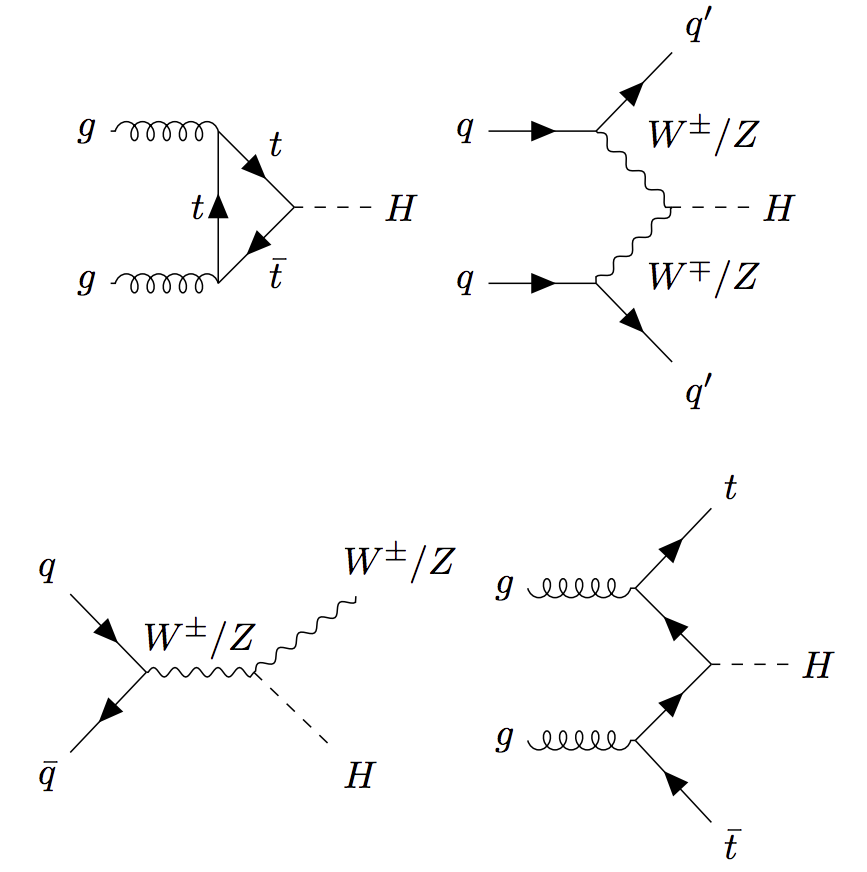
\includegraphics[width=0.7\textwidth]{Figures/Theory/FeynProd.png}
\caption{
  Feynman diagrams representing the four principal Higgs boson production modes at the LHC.
  In descending order of cross section, these are: ggH in the top left, VBF in the top right, 
  VH in the bottom left, and ttH in the bottom right.
}
\label{fig:theory_FeynProd}
\end{figure}

\subsection{Higgs boson decay modes}

The SM predicts that the Higgs boson has an extremely short lifetime~\cite{YR4}.
The Higgs boson is therefore never observed directly, 
but instead its presence is inferred from its decay products.
There are several permitted decay modes of the Higgs boson.
Since its coupling strength to other particles is proportional to the mass of the decay product, 
it can decay directly to any massive particle
\footnote{Only decays to pairs of particles whose mass is less than half that of the the Higgs boson
are permitted kinematically. 
However the decay can still occur to virtual particles of greater mass, 
which then themselves decay}.
In addition, loop diagrams permit the decay to massless particles, including the gluon and photon.
The branching fractions for each of the nine principal decay modes 
is shown in Table~\ref{tab:theory_decay}.
It can be seen that the decay to $b\bar{b}$ has the largest branching fraction.
However due to the large hadronic background at the LHC, 
this decay channel is very difficult to utilise experimentally.
The channels with the most sensitivity, despite their relatively low branching fractions, 
are the diphoton ($\gamma\gamma$) and $ZZ^{*}$ decays 
(where $Z^{*}$ indicates a virtual, or off mass-shell, Z boson).
The sensitivity of these channels depends on the relatively low background 
and the ability to precisely reconstruct the mass of the Higgs boson from the decay products.
The analyses of the $\gamma\gamma$ and $ZZ^{*}$ decay channels were the most important 
at the time of the discovery of the Higgs boson, 
and for the same reasons are now are ideally suited to the study of its properties.
This analysis uses the diphoton decay channel.
Three Feynman diagrams representing the largest contributions to the effective vertex 
between the Higgs boson and two photons are shown in Figure~\ref{fig:theory_FeynDecay}.
As can be seen in the figure, 
the decay to two photons is therefore sensitive to the Higgs boson's coupling to other particles, 
including the top quark and the W boson.

\begin{figure}[hptb]
\centering
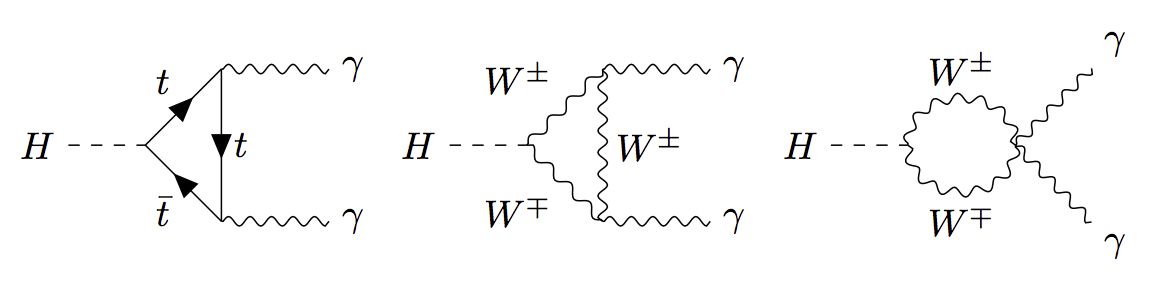
\includegraphics[width=\textwidth]{Figures/Theory/FeynDecay.png}
\caption{
  The Feynman diagrams with the largest contribution to the \Hgg decay loop.
}
\label{fig:theory_FeynDecay}
\end{figure}

\subsection{Status of Higgs boson measurements}

Since its discovery, remarkable progress has been made 
in measuring the properties of the Higgs boson.
Its mass is now known to a precision of better than 0.2\%~\cite{HIG-16-041}.
The rate of its production has also been measured precisely.
These measurements are usually parameterised as signal strength modifiers $\mu$,
which are defined as the ratio of the observed Higgs boson yield to the SM expectation.
This can be defined inclusively, for all Higgs boson production and decay modes, 
or for individual combinations of production and decay modes.
The general definition is written as
\begin{equation}
\mu^f_i = \frac{\sigma_i\mathcal{B}^f}{(\sigma_i)_{\textrm{SM}}(\mathcal{B}^f)_{\textrm{SM}}}
\end{equation}
where $\sigma_i$ and $\mathcal{B}^f$ are the observed production cross section 
and decay branching fraction respectively, 
and the ``SM" subscript refers to their respective SM predictions.

An example of signal strength modifier measurements 
from the previous CMS \Hgg analysis~\cite{HIG-16-040} is shown in Figure~\ref{fig:theory_PerProcTrad}.
The modifiers for the ggH, VBF, ttH and VH production processes and the diphoton decay are shown, 
with the inclusive diphoton decay modifier overlaid.
In this single decay channel with one experiment, 
the ggH signal strength is already measured to a precision of 20\%.
Combinations of results across different decay channels performed for optimal precision,
with the inclusive Higgs signal strength now measured 
to a precision of around 10\%~\cite{ATLAScomb,CMScomb}.
So far, all measurements are consistent with the SM predictions.

\begin{figure}[hptb]
\centering
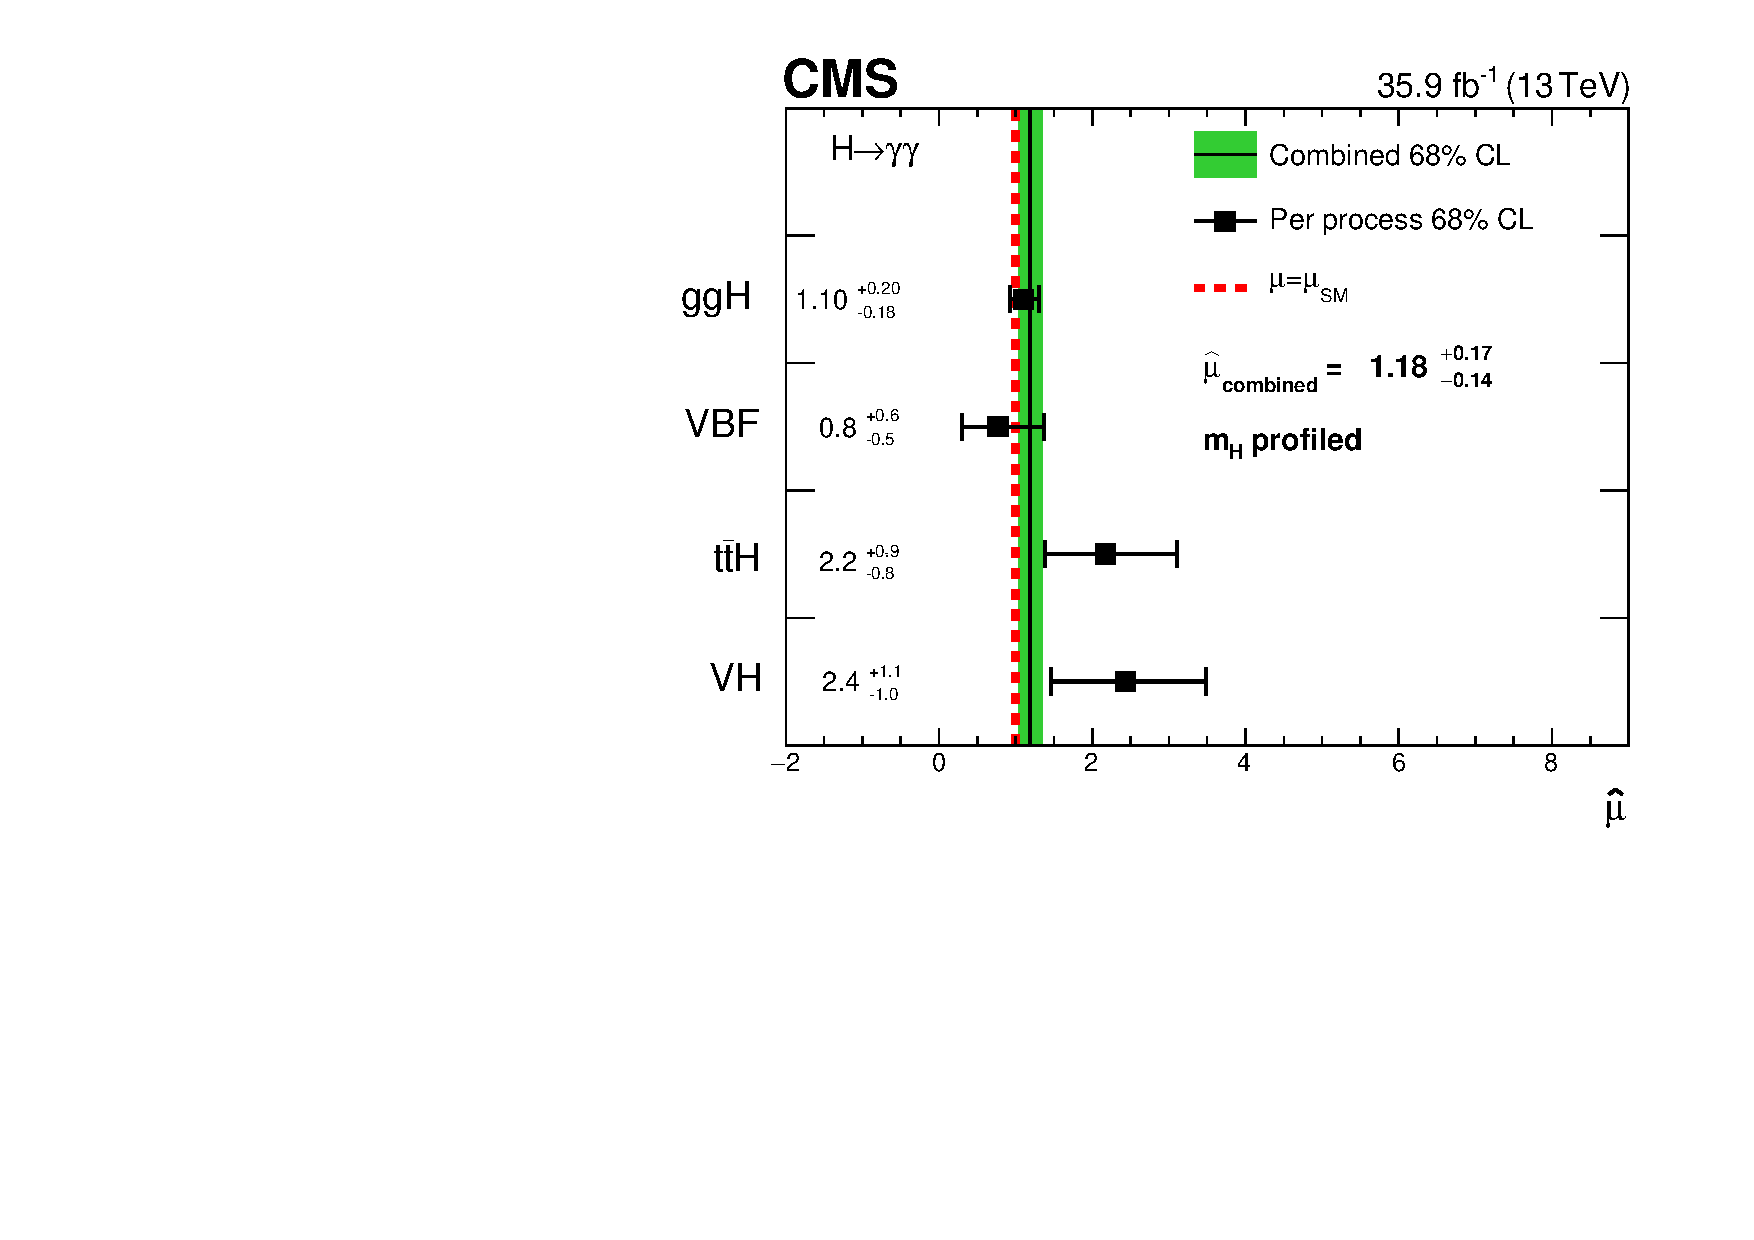
\includegraphics[width=0.8\textwidth]{Figures/Theory/PerProcTrad.pdf}
\caption{
  Signal strength modifier measurements in the \Hgg decay channel.
  The modifiers for each process (black points) are shown, with the SM Higgs boson mass profiled, 
  compared to the overall signal strength modifier (green band) 
  and to the SM expectation (dashed red line)
  Taken from Ref.~\cite{HIG-16-040}.
}
\label{fig:theory_PerProcTrad}
\end{figure}

\section{The simplified template cross section framework}

The simplified template cross section (STXS) framework \cite{YR4}
provides a coherent approach with which to perform precision Higgs boson measurements. 
Its goal is to minimise the theory-dependence of Higgs boson measurements, 
whilst permitting the use of advanced analysis techniques to optimise the measurements' sensitivity.
This also increases the reinterpretability of the measurements.
It is designed to supersede the traditional signal strength modifier measurements.

In the STXS framework, 
theoretically-motivated kinematic regions based upon Higgs boson production modes are defined.
These simplified regions, or bins, exist in varying degrees of granularity, 
following sequential ``stages".
At the so-called STXS stage 0, 
the bins correspond closely to the different Higgs boson production mechanisms.
An additional requirement is placed on the Higgs boson rapidity $|y_H| < 2.5$, 
which reduces the theoretical uncertainty 
that would otherwise arise when extrapolating measurements to the full phase space,
a large part of which is not accessible experimentally.
The experimental acceptance of \Hgg events with $|y_H| > 2.5$ is negligible.
The stage 0 bins are illustrated in Figure~\ref{fig:theory_stage0}.
The principal difference from the production proceses used in the signal strength measurements
is that VH production where the vector boson decays hadronically is grouped together with 
VBF production to define an ``electroweak qqH" bin.

%stage 0 bin definitions
\begin{figure}[hptb]
\centering
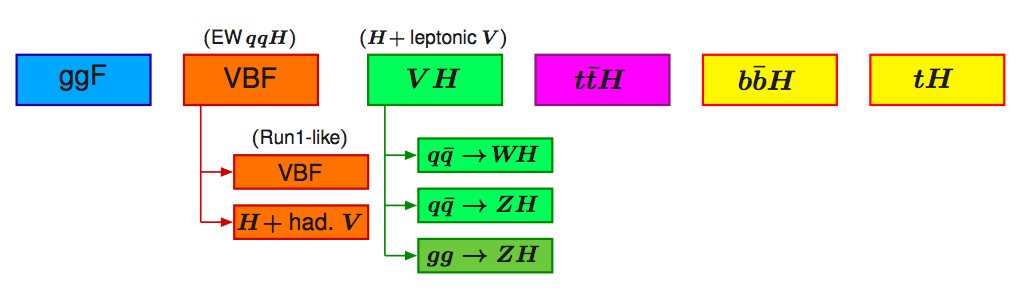
\includegraphics[width=0.8\textwidth]{Figures/Theory/stage0.png}
\caption{
  Taken from Ref.~\cite{YR4}.
}
\label{fig:theory_stage0}
\end{figure}

Measurements of stage 0 cross sections in the \Hgg decay channel 
were performed in the previous CMS \Hgg analysis~\cite{HIG-16-040}.
The results are shown in Figure~\ref{fig:theory_PerProcSTXS}, 
which is similar to Figure~\ref{fig:theory_PerProcTrad}.
Aside from the change in signal bin definitions and the absence of an inclusive measurement, 
the main difference is in the treatment of the theoretical uncertainties.
When performing a measurement of $\mu$, 
a fit is performed for the signal strength modifier ratio. 
This requires that the theoretical uncertainty on the SM prediction, 
which enters via the denominator, to be included.
In contrast if the fit parameter is only the observed cross section, 
the measurement does not depend on the overall SM prediction 
and this uncertainty does not need to be included.
It is instead considered as the uncertainty on the SM prediction, 
as displayed in Figure~\ref{fig:theory_PerProcSTXS}.
This separation of the theoretical uncertainties means that the measurement is less dependent 
on the theoretical prediction and remains useful 
even if improved theoretical predictions are obtained in the future.

\begin{figure}[hptb]
\centering
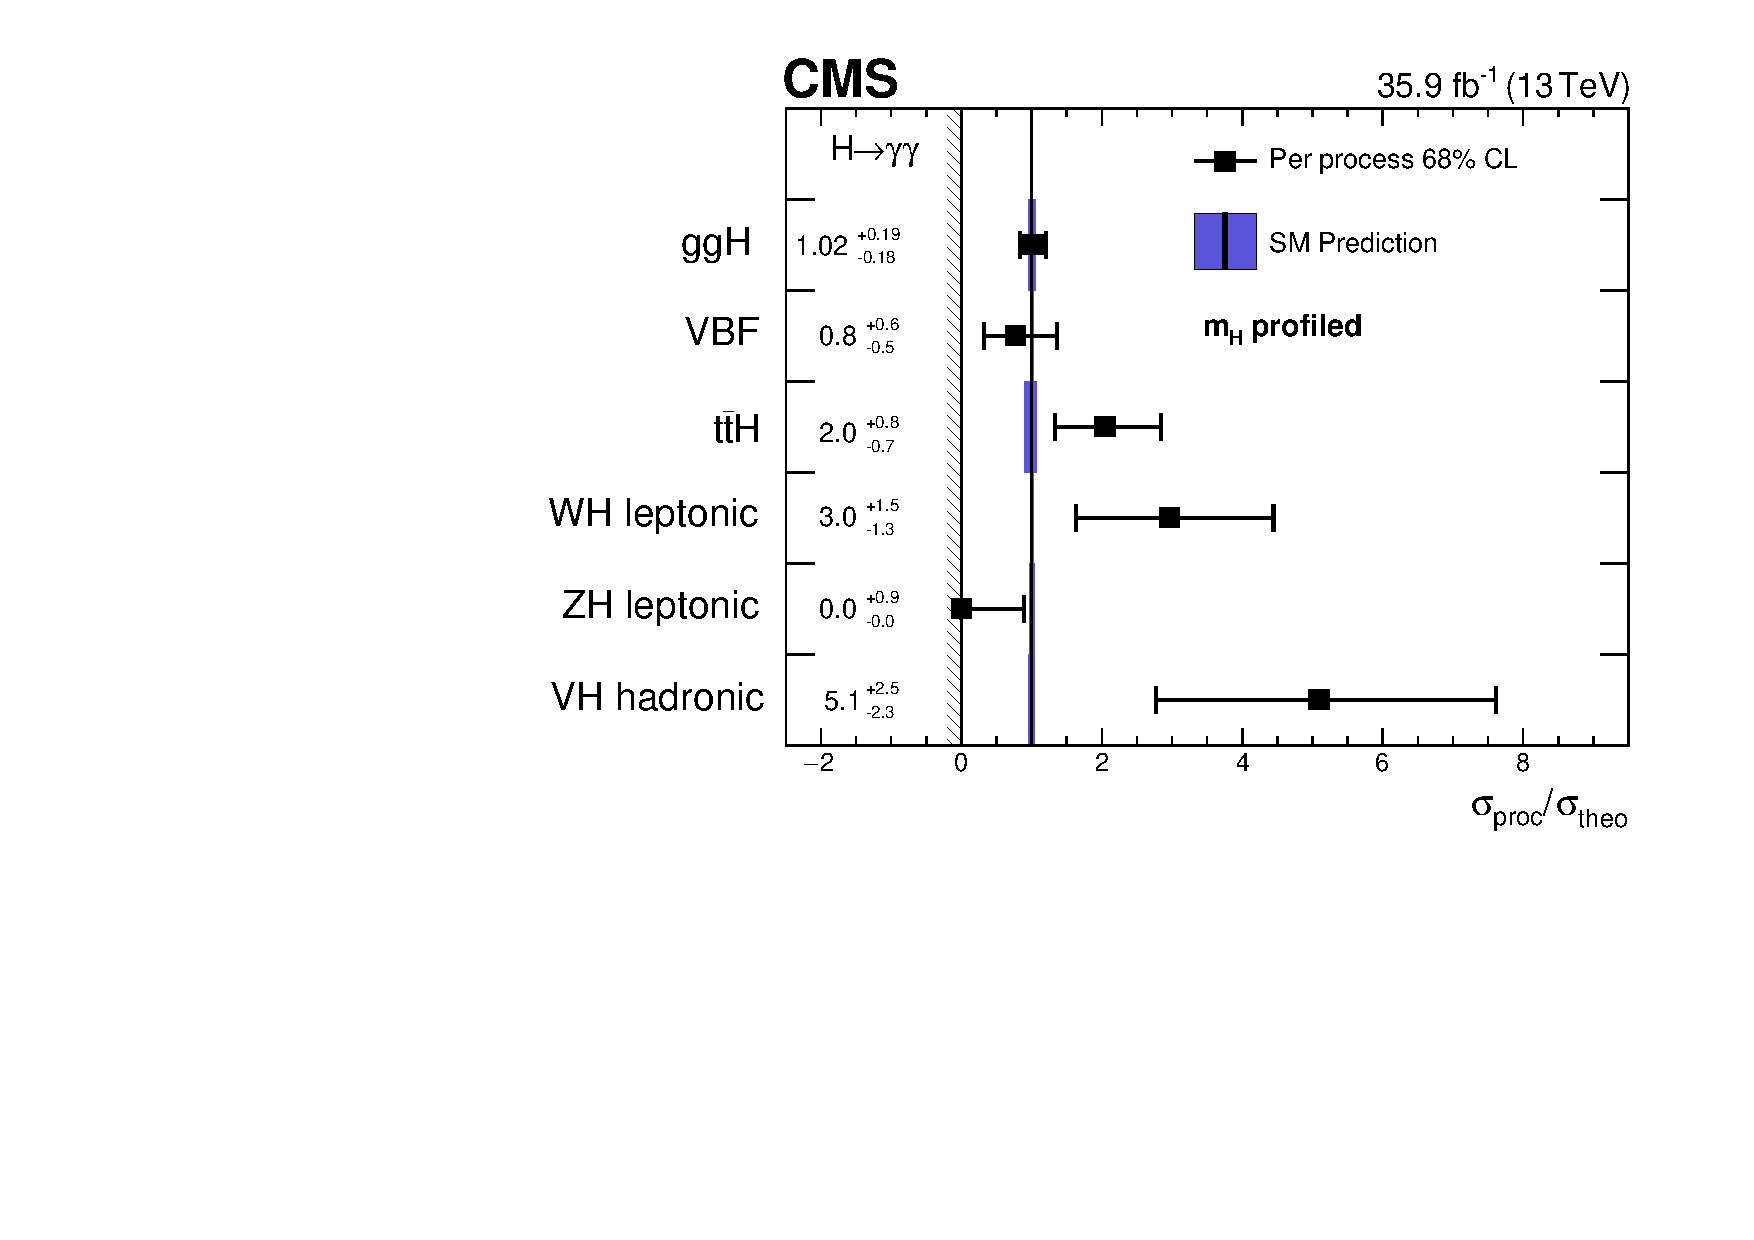
\includegraphics[width=0.8\textwidth]{Figures/Theory/PerProcSTXS.pdf}
\caption{
  Normalised cross sections measured for each stage 0 bin (black points) 
  in the Higgs simplified template cross section framework, 
  with the SM Higgs boson mass profiled, 
  compared to the SM expectations and their uncertainties (blue band). 
  The signal strength modifiers are constrained to be nonnegative, 
  as indicated by the vertical line and hashed pattern at zero.
  Taken from Ref.~\cite{HIG-16-040}.
}
\label{fig:theory_PerProcSTXS}
\end{figure}

At stage 1, a further splitting of bins into different kinematic regions is performed.
This provides additional information for different theoretical interpretations of the measurements, 
and enhances the sensitivity to possible signatures beyond the standard model (BSM).
Measurements at stage 1 of the framework have already been reported by the ATLAS Collaboration \cite{ATLAS_Hgg36,ATLAS_Hgg80,ATLASstage0_ZZ}; 
this analysis comprises the first CMS measurement of STXS stage 1 regions in the diphoton channel, 
covering the gluon fusion (ggH) and vector boson fusion (VBF) production modes.
The definitions of the different bins are shown in 
Figures~\ref{fig:theory_stage1ggH} and Figures~\ref{fig:theory_stage1VBF} 
for ggH and VBF production respectively.
For ggH production, bins are defined using the transverse momentum of the Higgs boson
and the number of jets in the event. 
In addition there are two bins for events with two jets where the event kinematics
resemble those of typical VBF events.
For VBF production, the bins are defined using the kinematics 
of the characteristic dijet system.
The ultimate goal of this analysis is to measure these bins as precisely as possible.
Further detail of the exact bin definitions 
and the methods used to discriminate between them is given in Chapter~\ref{chap:categorisation}.

%stage 1 bin definitions
\begin{figure}[hptb]
\centering
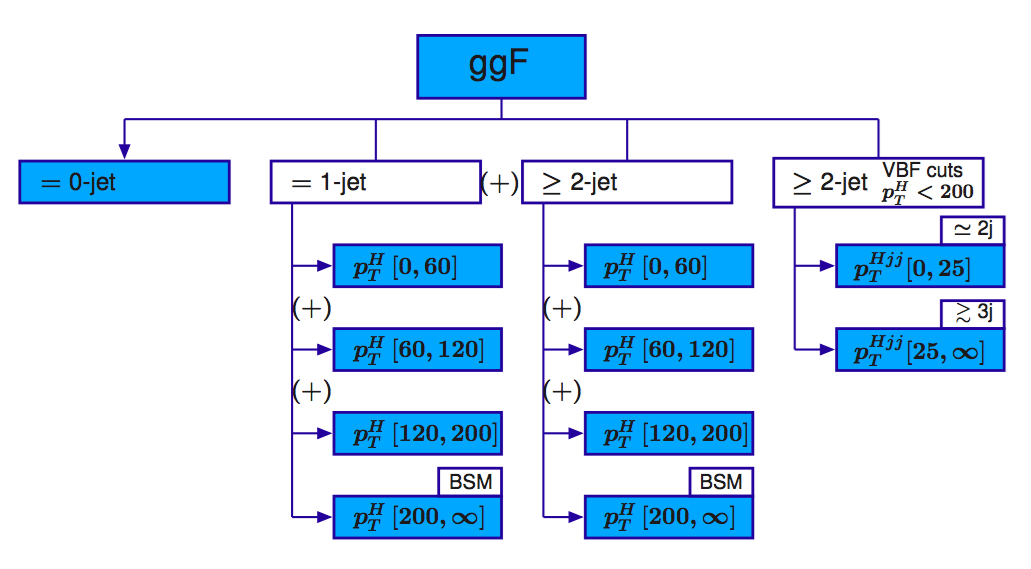
\includegraphics[width=0.8\textwidth]{Figures/Theory/stage1ggH.png}
\caption{
  The STXS stage 1 bins for the ggH production mode.
  Taken from Ref.~\cite{YR4}.
}
\label{fig:theory_stage1ggH}
\end{figure}

\begin{figure}[hptb]
\centering
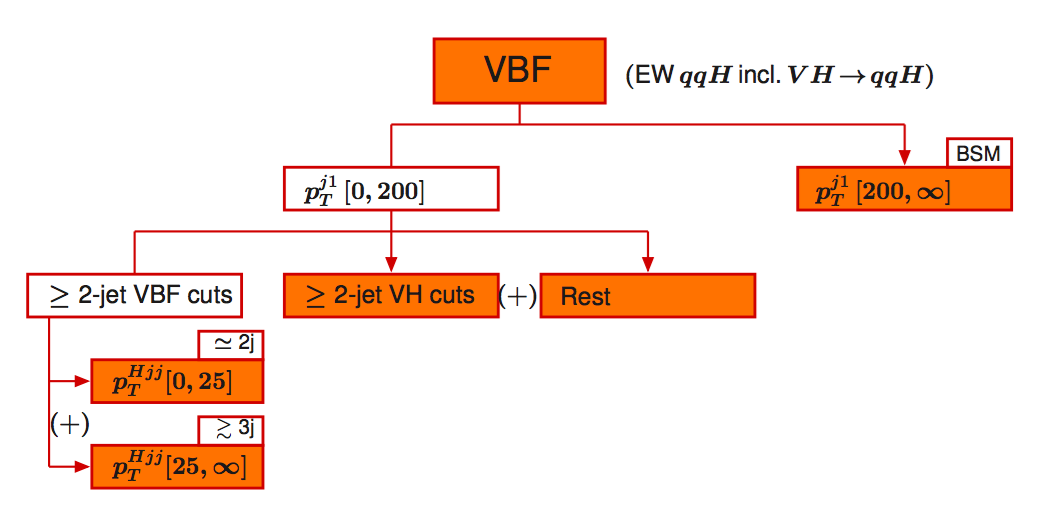
\includegraphics[width=0.8\textwidth]{Figures/Theory/stage1VBF.png}
\caption{
  The STXS stage 1 bins for the VBF production mode.
  Taken from Ref.~\cite{YR4}.
}
\label{fig:theory_stage1VBF}
\end{figure}
